\documentclass[12pt,letterpaper]{article}
\usepackage[lmargin=1in,rmargin=1in,tmargin=1in,bmargin=1in]{geometry}
\usepackage{exams}

% -------------------
% Content
% -------------------
\begin{document}
\coverpage{MAT 999: Section \#\#\#}{Semester Year}{Exam 1}

% Instructions
\noindent This exam has \total{problem} problems on \pageref{LastPage} pages. There are no calculators, phones, or other electronic devices allowed during this exam. Be sure to show all your work. \vspace{1cm}

% Name & Score
\namescoreline


% Question 1
\problem This is a numbered problem. \vspace{3cm}



% Question 2
\problem This is the second numbered problem. \vfill



% Question 3
\problem Choosing an answer to this questions at random, what is the chance that it will be correct?
	\begin{enumerate}[(a)]
	\item 25\%
	\item 50\%
	\item 70\%
	\item 25\%
	\end{enumerate} \vfill



\newpage



% Question 4
\problem Solve the Riemann Hypothesis. Be sure to justify each step.



% Question 5
\newpage
\problem Write an answer to an unasked question in the space below. \pspace
\emptybox{2in}



% Question 6
\newpage
\problem Write an award winning level novel in the space below. \pspace
\emptybox{8in}



% Question 7
\newpage
\problem Choose an option.
	\begin{enumerate}[(a)]
	\item Here is an option.
	\item Here is another.
	\item A third choice!
	\end{enumerate}



% Question 8
\newpage
\problem Answer the following parts completely. \vspace{0.5cm}
	\begin{enumerate}[(a)]
	\item What is Mathematics? \vspace{2cm}
	\item Why are we here? \vfill
	\item What is the meaning of life? \vfill
	\end{enumerate}
	
	
	
% Question 9
\newpage
{%
	% Defines choice options: \roman, \arabic, etc
%	\renewcommand*\thechoice{\roman{choice}}
%	\renewcommand*\itemlabel{\thechoice)}
\problem What is $2+2=$ ?
	\begin{multicols}{2}
	\begin{enumerate}[(a)]
	\item Martha Washington
	\item Mars
	\item 17
	\item 4
	\item $-4$
	\item Cannot be determined.
	\item None of the above.
	\item All of the above.
	\end{enumerate}
	\end{multicols}
}%



% Question 10
\newpage
\problem Draw a graph below. 
	\[
	\begin{tikzpicture}
	\tkzInit[xmax=7,ymax=7,xmin= -7,ymin= -7]
   	\tkzGrid
   	\tkzAxeXY
  	\end{tikzpicture}
	\]



% Question 11
\newpage
\problem Draw a graph below.
	\[
	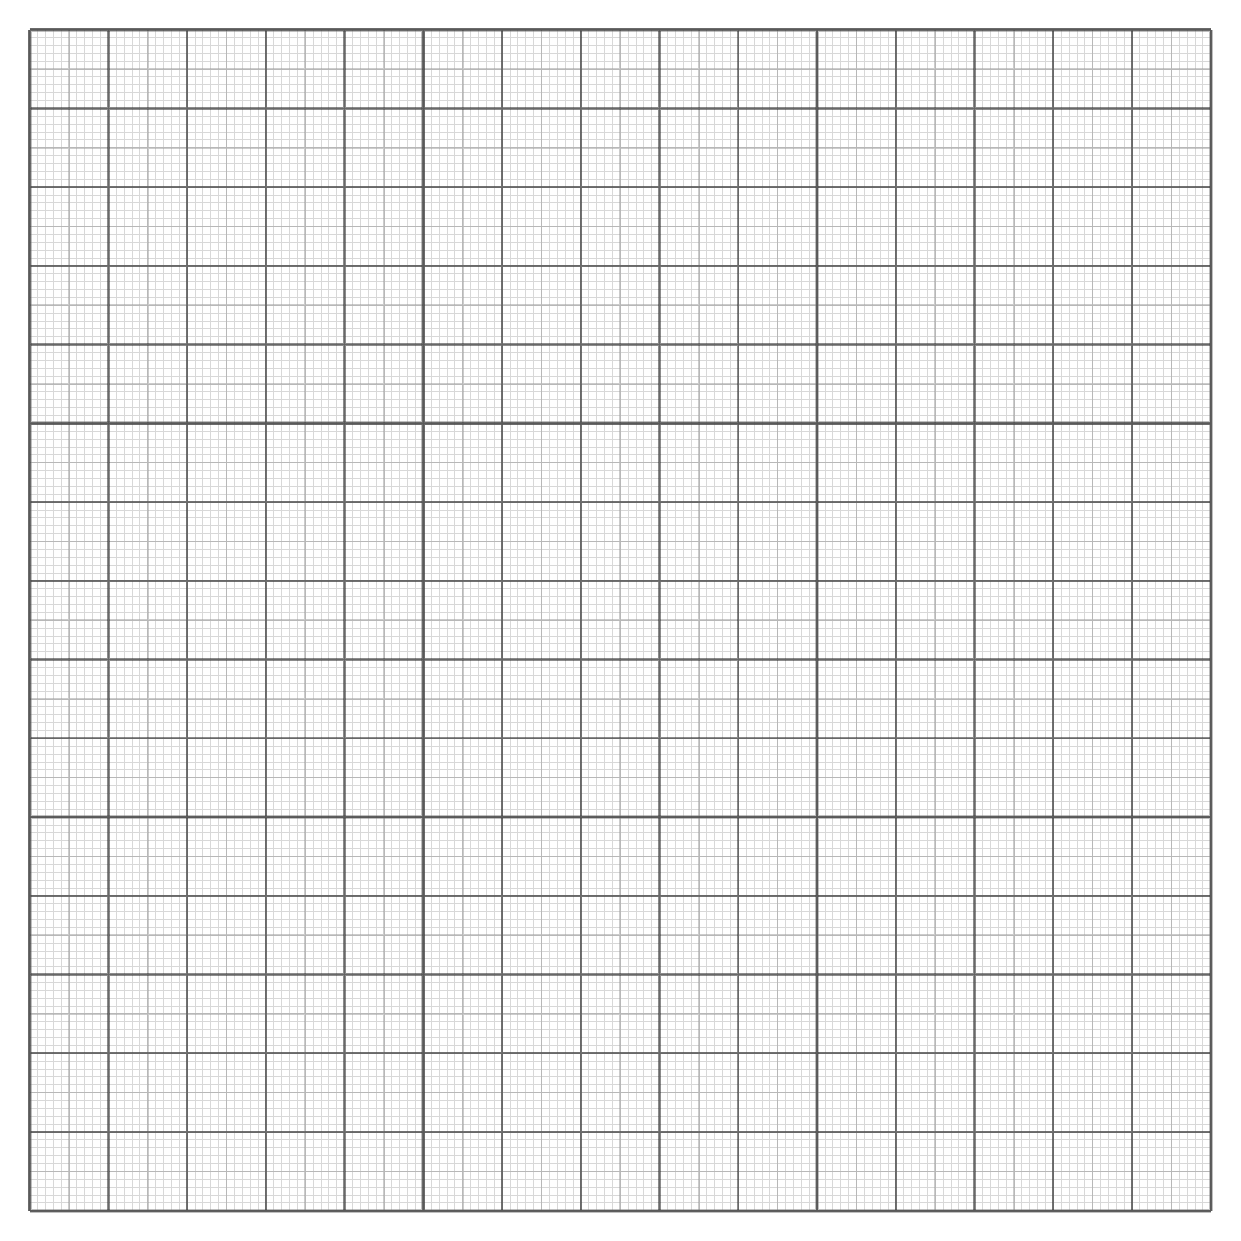
\begin{tikzpicture}[x=1cm, y=1cm, semitransparent]
	\draw[step=1mm, line width=0.1mm, black!30!white] (0,0) grid (15,15);
	\draw[step=5mm, line width=0.2mm, black!40!white] (0,0) grid (15,15);
	\draw[step=5cm, line width=0.5mm, black!50!white] (0,0) grid (15,15);
	\draw[step=1cm, line width=0.3mm, black!90!white] (0,0) grid (15,15);
	\end{tikzpicture}
	\]



\end{document}